\documentclass[main.tex]{subfiles}
\begin{document}

\chapter{Oefenzittingen}
\label{cha:oefenzittingen}

\section{Oefenzitting 1}
\label{sec:oz1}

\subsection*{Oefening 1}
$T_{p}\mathbb{A}^{n}$ is inderdaad een vectorruimte.\footnote{Zie stelling \ref{st:rakende-ruimte-is-vectorruimte}.}
$\phi$ is inderdaad een isomorfisme van re\"ele vectorruimten.\footnote{Zie stelling \ref{st:phi-isomorphisme}.}

\subsection*{Oefening 2}

\begin{itemize}
\item Nee, $V$ en $W$ zijn ongelijk want $(1,2)$ is lineair onafhankelijk van $(0,-2)$.
\item $q + V$.
\item $p + W$
\end{itemize}

\subsection*{Oefening 3}
\begin{enumerate}
\item $p+V$ en $q+W$
  \[
  \begin{vmatrix}
    1 & 1 & 1\\
    0 & 2 & 4\\
    1 & 3 & 5
  \end{vmatrix}
  = 0
  \Rightarrow W \subsetneq V 
  \]
  $q+W$ is dus zwak parallel met $p+V$.
  \[ p+W \triangleleft q+V \]
\item $p+V$ en $q+R$
  \[
  \begin{vmatrix}
    2 & 9 & 1\\
    2 & 2 & 4\\
    4 & 2 & 5
  \end{vmatrix}
  = 0
  \Rightarrow W \subsetneq R 
  \]
  $p+W$ is dus zwak parallel met $q+R$.
  \[ p+W \triangleleft q+R \]
  
\item $q+W$ en $q+R$
  \[
  \begin{vmatrix}
    1 & 0 & 1\\
    1 & 2 & 3\\
    2 & 2 & 4
  \end{vmatrix}
  = 0
  \text{ en }
  \begin{vmatrix}
    1 & 0 & 1\\
    1 & 2 & 3\\
    0 & 2 & 2
  \end{vmatrix}
  = 0
  \Rightarrow V = R
  \]
  $q+W$ en $q+R$ zijn dus parallel.
  \[ q+W \parallel q+R \]
\end{enumerate}

\extra{oefening 4}

\subsection*{Oefening 5}
\[ S + T = p + (V + W) = p + <\{(1,0,0),(0,1,0)\}>\]

\subsection*{Oefening 6}
Zie stelling \ref{st:affiene-deelruimten-niet-lege-doorsnede-gelijk}

\subsection*{Oefening 7}
We maken een gevalsonderscheid.
\begin{itemize}
\item $(s,t)$ met $s$ of $t$ groter of gelijk aan $n$ kan geen oplossing zijn want dan zou $S$ of $T$ geen deelruimte zijn van $\mathbb{A}^{n}$.
\item $(n-1,n-1)$ kan wel:
  Kies een $n-1$ dimensionale affiene deelruimte $S = p + V$ van $\mathbb{A}^{n}$.
  Er zit nu minstens \'e\'en punt $q\in \mathbb{A}^{n}$ niet in $S$.
  Beschouw nu de $n-1$ dimensionale affiene deelruimte $T = q + V$.
  $S$ en $T$ zijn parallel en niet gelijk, dus disjunct.\footnote{Zie stelling \ref{st:parallelle-deelruimten-gelijk-of-disjunct}.}
\item $(s,t)$ met $s,t < n-1$ kan ook.
  Beschouw immers een $s$ en $t$ dimensionale deelruimnten van $S$ en $T$ uit het bovenstaande puntje.
  Deze deelruimten zijn nog steeds disjunct.
\end{itemize}
Antwoord:
\[ \{(s,t)\in \mathbb{N}\times\mathbb{N}\ |\ s,t<n\}\]

\subsection*{Oefening 8}
$S$ en $T$ zijn kruisend.
\begin{enumerate}
\item Stel $S = s+V$ en $T = t+W$.
  Beschouw nu $R_{1} = s + (V+W)$
  $R_{1}$ is nu zwak parallel met $T$ want $W \subsetneq (V+W)$.
  $R_{1}$ is bovendien uniek, want stel dat er twee verschillende vlakken $R_{1}$ en $R_{1}'$ zijn die $S$ bevatten en zwak parallel zijn met $T$, dan is $W$ een deelverzameling van zowel de richting van $R_{1}$ als de richting van $R_{1}'$. Bovendien zou $s$ een element zijn van zowel $R_{1}$ als $R_{1}'$, en zouden bijgevolg $R_{1}$ en $R_{1}'$ gelijk zijn.\footnote{Zie stelling \ref{st:zwak-parallelle-deelruimten-deel-of-disjunct}.}
\item Volledig analoog.
\item $R_{1} = s + (V+W)$ en $R_{1} = t + (V+W)$, hebben dezelfde richting en dimensie, en zijn bijgevolg parallel.
\end{enumerate}

\extra{oefening 9}
 
\subsection*{Oefening 10}
Tegenvoorbeeld:
Kies $S = <e_{1},e_{2}>$ en $T = <e_{3},e_{4}>$ deelruimten van $\mathbb{A}^{4}$.


\section{Oefenzitting 2}
\label{sec:oefenzitting-2}

\subsection*{Oefening 1}
Bepaal de parametervergelijkingen en carthesische vergelijkingen van de rechte door $p$ en $q$:
\begin{enumerate}
\item 
\extra{oefening 1.1}
\item
\extra{oefening 1.2}
\item
\extra{oefening 1.3}
\item $p = (2,-1,7)$ en $q=(6,4,-3)$ in $\mathbb{A}^{3}$\\
  \[ \overrightarrow{pq} = (6,4,-3) - (2,-1,7) = (4,5,-10) \]
  Parametervergelijkingen:
  \[ L \leftrightarrow x \in p + <\overrightarrow{pq}> \]
  \[ L \leftrightarrow x = (2,-1,7) + \lambda(4,5,-10) \]
  Carthesische vergelijkingen:
  \[
  L \leftrightarrow
  rang
  \begin{pmatrix}
    (x_{1}-2) & (x_{2}+1) & (x_{3}-7)\\
    4 & 5 & -10
  \end{pmatrix}
  = 1 = dim(rechte)
  \]
  \[
  \Leftrightarrow 
  \begin{vmatrix}
    (x_{1}-2) & (x_{2}+1)\\
    4 & 5
  \end{vmatrix}
  = 0
  \wedge
  \begin{vmatrix}
    (x_{2}+1) & (x_{3}-7)\\
    5 & -10
  \end{vmatrix}
  = 0
  \]
  \[ v_{1}(x_{i}-p_{i}) = v_{i}(x_{1}-p_{1}) \]
  $\rightarrow$
  \[
  \left\{
    \begin{array}{ccc}
      4(x_{2}+1) &=& 5(x_{1}-2)\\
      4(x_{3}-7) &=& -10(x_{1}-2)
    \end{array}
  \right.
  \leftrightarrow
  \left\{
    \begin{array}{ccccc}
      5x_{1}&-4x_{2}&&=&14\\
      5x_{1}&&+2x_{3}&=&24
    \end{array}
  \right.
  \]
\item
\extra{oefening 1.5}
\end{enumerate}

\subsection*{Oefening 2}
Bepaal parametervergelijkingen en carthesische vergelijkingen van het vlak door $p$, $q$ en $r$ in de volgende gevallen.
\begin{enumerate}
\item $p=(0,1,1)$, $q=(1,-1,1)$ en $r=(3,-2,4)$ in $\mathbb{A}^{3}$\\
  \[ \overrightarrow{pq} = (1,-1,1) - (0,1,1) = (1,-2,0) \]
  \[ \overrightarrow{pr} = (3,-2,4) - (0,1,1) = (3,-3,3) \]
  Parametervergelijkingen:
  \[ H \leftrightarrow x = (0,1,1) + \lambda (1,-2,0) + \mu (3,-3,3) \]
  Carthesische vergelijkingen:
  \[
  H \leftrightarrow 
  rang 
  \begin{pmatrix}
    x_{1} & (x_{2}-1) & (x_{3}-1)\\
    1 & -2 & 0\\
    1&-1&1
  \end{pmatrix}
  = 2 = dim(vlak)
  \]
  \[
  \Leftrightarrow 
  \begin{vmatrix}
    x_{1} & (x_{2}-1) & (x_{3}-1)\\
    1 & -2 & 0\\
    1&-1&1
  \end{vmatrix}
  = 0
  \]
  \[ H \leftrightarrow 2x_{1}+ x_{2}-x_{3} = 0 \]
\extra{oefening 2.1}
\item $p= (1,0,6,1)$, $q=(2,-1,3,7)$ en $r=(0,0,2,1)$ in $\mathbb{A}^{4}$\\
  \[ \overrightarrow{pq} = (2,-1,3,7) - (1,0,6,1) = (1,-1,-3,6) \]
  \[ \overrightarrow{pr} = (0,0,2,1) - (1,0,6,1) = (1,0,-4,0) \]
\extra{oefening 2.2}
  
\end{enumerate}

\subsection*{Oefening 3}
Bepaal parametervergelijkingen en carthesische vergelijkingen van de affiene deelruimten $H$ bepaald door de volgende punten.
\begin{itemize}
\item $p_{0} = (1,0,0,0)$, $p_{1} = (0,1,1,2)$, $p_{2} = (0,0,0,0)$ en $p_{3} = (1,2,3,4)$ in $\mathbb{A}^{4}$\\
  \[ \overrightarrow{p_{1}p_{2}} = (0,1,1,2) - (1,0,0,0) = (-1,1,1,2) \]
  \[ \overrightarrow{p_{1}p_{3}} = (0,0,0,0) - (1,0,0,0) = (-1,0,0,0) \]
  \[ \overrightarrow{p_{1}p_{4}} = (1,2,3,4) - (1,0,0,0) = (0,2,3,4) \]
  Parametervergelijkingen:
  \[ H \leftrightarrow x = (1,0,0,0) + \lambda(-1,1,1,2) + \mu(-1,0,0,0) + \nu(0,2,3,4) \]
  Carthesische vergelijkingen:
  \[
  H \leftrightarrow
  rang
  \begin{pmatrix}
    x_{1} & x_{2} & x_{3} & x_{4}\\
    1 & 2 & 3 & 4\\
    1 & 0 & 0 & 0\\
    0 & 1 & 1 & 2\\
  \end{pmatrix}
  = 3
  \]
  \[
  \Leftrightarrow
  \begin{vmatrix}
    x_{1} & x_{2} & x_{3} & x_{4}\\
    1 & 2 & 3 & 4\\
    1 & 0 & 0 & 0\\
    0 & 1 & 1 & 2\\
  \end{vmatrix}
  = 
  \begin{vmatrix}
    x_{2} & x_{3} & x_{4}\\
    2 & 3 & 4\\
    1 & 1 & 2\\
  \end{vmatrix}
  = 0
  \]
  \[
  H \leftrightarrow 2x_{2} - x_{4} = 0
  \]
\item 
  \extra{ oefening 3.2 }
\end{itemize}

\subsection*{Oefening 4}
  \extra{ oefening 4 }
\subsection*{Oefening 5}
Gegeven een is volgend stelsel vergelijkingen.
\[
\left\{
  \begin{array}{cc}
    1 + x_{1} + x_{2} - x_{3} - 6x_{4} &= 0\\
    1 - x_{1} + 2x_{2} - x_{3} - 2x_{4} &= 0\\
    1 - 3x_{1} + 3x_{2} - x_{3} + 2x_{4} &= 0
  \end{array}
\right.
\]
\begin{itemize}
\item Wat is de dimensie van de bijhorende affiene deelruimte $H$ van $\mathbb{A}^{4}$?
\item Geef de Parametervergelijkingen voor deze affiene deelruimte.
\end{itemize}

\[ 
A = 
\begin{pmatrix}
    1 & 1 & -1 & -6 & -1\\
    -1 & 2 & -1 & -2 & -1\\
    -3 & 3 & -1 & 2 & -1
\end{pmatrix}
\rightarrow
\begin{pmatrix}
  1 & 0 & -\frac{1}{3} & -\frac{10}{3} & -\frac{1}{3}\\
  0 & 1 & -\frac{2}{3} & -\frac{8}{3}  & -\frac{2}{3}\\
  0 & 0 & 0            & 0             & 0
\end{pmatrix}
\] 
\begin{itemize}
\item $dim(H) = n - rang(A) = 4 - 2 = 2$.
\item Stelsel oplossen:
  \[
  \left\{
  \begin{array}{cl}
    x_{1} &= -\frac{1}{3} \lambda + -\frac{10}{3} \mu -\frac{1}{3}\\
    x_{2} &= -\frac{2}{3} \lambda + -\frac{8}{3}  \mu -\frac{2}{3}\\
    x_{3} &= \lambda\\
    x_{4} &= \mu
  \end{array}
  \right.
  \]
  \[ H \leftrightarrow x = \left(-\frac{1}{3},-\frac{2}{3},0,0-\right) + \lambda\left(-\frac{1}{3},-\frac{2}{3},1,0\right) + \mu\left(-\frac{10}{3},-\frac{8}{3},0,1\right) \]
\end{itemize}

\subsection*{Oefening 6}
Gegeven is de rechte $L$ in $\mathbb{A}^{3}$.
\[ 
\left\{
  \begin{array}{cc}
    x + y - z + 7 = 0\\
    2x - y + z + 8 = 0
  \end{array}
\right.
\]
\begin{enumerate}
\item Geef de richting van $L$.\\
  Het volgende homogeen stelsel geeft ons de richting van $L$ in zijn oplossing:
\[ 
\left\{
  \begin{array}{cc}
    x + y - z = 0\\
    2x - y + z = 0
  \end{array}
\right.
\]
\[
\begin{pmatrix}
  1 & 1 & -1 & 0\\
  2 & -1 & 1 & 0
\end{pmatrix}
\rightarrow
\begin{pmatrix}
  1 & 0 & 0  & 0\\
  0 & 1 & -1 & 0
\end{pmatrix}
\]
De richting van $L$ is dus $V$:
\[
V = \{ (0,-\lambda,\lambda)\ |\ \lambda \in \mathbb{R}^{3} \} 
\]
\item Bepaal de rechte $L'$ door het punt $p = (-1,2,0)$ parallel met $L$.\\
\[ L' = p + V = (-1,2,0) + \lambda (0,-1,1) \]
OF bepaal $a$ en $b$ in volgend stelsel voor de carthesische vergelijkingen door $p$ in te vullen.
\[ 
\left\{
  \begin{array}{cc}
    x + y - z + a = 0\\
    2x - y + z + b = 0
  \end{array}
\right.
\rightarrow 
\left\{
  \begin{array}{cc}
    a = -1\\
    b = 4
  \end{array}
\right.
\]
Dan krijgen we volgende carthesische vergelijkingen voor $L$:
\[ 
\left\{
  \begin{array}{cc}
    x + y - z  -1 = 0\\
    2x - y + z + 4 = 0
  \end{array}
\right.
\]
\end{enumerate}

\subsection*{Oefening 7}
Gegeven zijn de rechten $L$ en $L'$ in $\mathbb{A}^{3}$ met als vergelijkingen:
\[
L = 
\left\{
\begin{array}{cl}
x + 2y + 3z &= 3\\
2x -y -z &= 1    
\end{array}
\right.
\quad\text{ en }\quad
L' = 
\left\{
\begin{array}{cl}
x - y - z &= -4\\
4x +2y -z &= 2
\end{array}
\right.
\]
\begin{itemize}
\item Toon aan dat deze rechten kruisend zijn.\\
We berekenen de doorsnede van $L$ en $L'$ door de vergelijkingen samen te nemen.
\[
\left\{
\begin{array}{cl}
x + 2y + 3z &= 3\\
2x -y -z &= 1\\
x - y - z &= -4\\
4x +2y -z &= 2
\end{array}
\right.
\]
\[
\rightarrow
\begin{pmatrix}
  1 & 2 & 3 & 3\\
  0 &-5 &-7 &-5\\
  0 & 0 & 1 & -20\\
  0 & 0 &-5 & 4
\end{pmatrix}
\]
We zien dat dit stelsel strijdig is, en de doorsnede bijgevolg leeg is.
\[ L \leftrightarrow x = (1,1,0) + \lambda(1,7,-5) \]
\[ L' \leftrightarrow x = (-1,3,0) + \lambda(1,-1,2) \]
We zien dat de rechten een verschillende righting hebben, dus ze zijn kruisend.

\item Bepaal de rechte met richting $(0,1,-1)$ die deze rechten snijdt.\\
Zij $H_{1}$ het vlak dat $L$ bevat en ook de richting $(0,1,-1)$ heeft.
\[ H_{1} \leftrightarrow x = (1,1,0) + \lambda(1,7,-5) + \mu (0,1,-1) \]
We zoeken dan het snijpunt $p$ van $H_{1}$ en $L_{2}$, dat is een punt op $L_{3}$.
\[ (-1,3,0) + \nu(1,-1,2) = (1,1,0) + \lambda(1,7,-5) + \mu (0,1,-1) \]
\[
\rightarrow
\begin{pmatrix}
  1 & 0 &-1 &-2\\
  7 & 1 & 1 & 2\\
  -5 &-1 &-2 & 0
\end{pmatrix}
\leftrightarrow
\begin{pmatrix}
  1 & 0 &-1 &-2\\
  7 & 1 & 1 & 3\\
  5 &-1 &-2 & 0
\end{pmatrix}
\]
De oplossing van dit stelsel is $(\lambda,\mu,\nu) = (4,-32,6)$ dus het snijpunt vinden we als volgt:
\[ (-1,3,0) + 6(1,-1,2) = (5,-3,12) \]
We kennen dan de richting van $L_{3}$ en een aangrijpingspunt van $L_{3}$.
\[ L_{3} = (5,-3,12) + \lambda (0,1,-1) \]
\end{itemize}

\extra{Oefening 8}
\extra{Oefening 9}
\extra{Oefening 10}
\extra{Oefening 11}
\extra{Oefening 12}

\section{Oefenzitting 3}
\extra{Oefening 1}

\subsection*{Oefening 2}
Gegeven zijn de homothetie $H_{c,r}$ met centrum $c$ en factor $r$, en de translatie $t_{a}$ in de richting van $a$.
Toon aan dat de samenstelling van $H_{c,r}$ en $t_{a}$ commutatief is.
\[ H_{c,r} \circ t_{a} = t_{a} \circ H_{c,r} \]
Noteer de definities van deze transformaties:
\[ 
\begin{array}{rl}
  H_{c,r}: & p \mapsto c + r\overrightarrow{cp}\\
  t_{a}:   & p \mapsto p + a\\
\end{array}
\]
Bekijk nu de samenstelling.
\[ 
\begin{array}{rll}
  H_{c,r} \circ t_{a} &= c + r\overrightarrow{c(p+a)} &\\
                     &= c + r(p + a - c) &\\
                     &= c + r\overrightarrow{pc} +ra &= t_{a} \circ H_{c,r}
\end{array}
\]

\subsection*{Oefening 3}
Zij $D$ een dilatatie van $\mathbb{A}^{n}$ en $l$ en $m$ twee rechten in $\mathbb{A^{n}}$ met snijpunt $P$.
\[ l \cap m = \{P\}\]
Stel dat er een punt $X$ op $l$ en een punt $Y$ op $m$ zodat $D(X)$ op $l$ ligt en $D(Y)$ op $m$.
Toon aan dat $P$ dan een vast punt is van $D$.
\[ (\exists x\in l,y\in m: (D(X) \in l) \wedge (D(Y) \in m)) \Rightarrow D(P) \]
\begin{proof}
  Elke dilatatie beeldt een affiene deelruimte af op een parallelle affiene deelruimte.\footnote{Zie stelling \ref{st:dilatatie-parallelle-deelruimte}.}
  $D(X)$ ligt op $l$, en wordt ook op een parallelle rechte afgebeeldt, dus moet die parallelle rechte $l$ zelf zijn.
  Een analoge redenering geldt voor$D(Y)$ en $m$.
  $D(P)$ wordt afgebeeldt op zowel $l$ als $m$, en dus op een punt in de doorsnede.
  De doorsnede $l\cap m$ bevat enkel $P$, dus $P$ wordt op zichzelf afgebeeld door $D$.
  \[ D(P) = P \]
\end{proof}

\subsection*{Oefening 4}
Gegeven zijn de homothetie\"en $H_{c,r}$ en $H_{d,r}$ van $\mathbb{A}^{n}$ met centra $c$ en $d$ en factoren $r$ en $s$.
\begin{itemize}
\item Toon aan dat $H_{c,r} \circ H_{d,s}$ een translatie is als en slechts als $rs = 1$ geldt.
\item Geef de nodige voorwaarden opdat $H_{c,r} \circ H_{d,s} = I_{\mathbb{A}^{n}}$ geldt. 
\end{itemize}
Noteer eerst de definities van $H_{c,r}$ en $H_{d,r}$.
\[
\begin{array}{rl}
  H_{c,r}: & p \mapsto c + r\overrightarrow{cp}\\
  H_{d.s}: & p \mapsto d + s\overrightarrow{dp}\\ 
\end{array}
\]
\begin{itemize}
\item Bekijk de samenstelling $H_{c,r} \circ H_{d,s}$.
\[
\begin{array}{rl}
  H_{c,r} \circ H_{d,s} &= c + r\overrightarrow{c(d+s\overrightarrow{dp})}\\
                      &= c + r(d + s\overrightarrow{dp} - c)\\
                      &= c + r(d + s(p-d) -c)\\
                      &= c + rd + rsp -rd -rc \\
                      &= rsp + (1-r)c + (1-s)rd\\
\end{array}
\] 
We zien dat dit laatste een translatie is als en slechs als de co\"efficient $rs$ bij $p$ $1$ is.
\end{itemize}
\extra{Oefening 5}

\subsection*{Oefening 6}
Stel dat een affiene transformatie $F$ elke affiene deelruimte afbeeldt op een parallele affiene deelruimte.
Toon aan dat $F$ een dilatatie is.\\\\
Inderdaad, zie stelling \ref{st:dilatatie-parallelle-deelruimte}.



\subsection*{Oefening 7}
Gegeven zijn $k+1$ affien onafhankelijke punten $p_{i}$ van $\mathbb{A}^{n}$ en een punt $p$ in de affiene deelruimte bepaald door deze punten.
Toon aan dat de barycentrische co\"ordinaten van $p$ ten opzichte van de punten $p_{i}$ invariant zijn onder affiene transformaties.
\[ \forall F:\ F(p) = \sum_{i=0}^{n}\lambda_{i}F(p_{i}) \]
\clarify{Waarom is dit belangrijk en niet gewoon saai? affiene meetkunde is de studie van verhoudingen. Lineaire algebra is...}
\begin{proof}
  Gegeven is het volgende:\footnote{Zie definitie \ref{barycentrische-coordinaten}.}
  \[ p = \sum_{i=0}^{k}\lambda_{i}p_{i} \quad\text{ met }\quad \sum_{i=0}^{k}\lambda_{i} = 1 \]
  Kies nu een willekeurige affiene transformatie $F$:
  \[ F: p\mapsto Ap + b \]
  \[
  \begin{array}{rll}
    F(p) &= A\sum_{i=0}^{k}\lambda_{i}p_{i} + b &\\
         &= \sum_{i=0}^{k}\lambda_{i}Ap_{i} + b &= \sum_{i=0}^{k}\lambda_{i}(Ap_{i} + b) 
  \end{array}
  \]
  Merk op dat die laatste stap alleen maar geldt als de $\lambda_{i}$ sommeren tot $1$.
\end{proof}

\section{Oefenzitting 4}
\label{sec:oefenzitting-4}

\extra{Oefening 1}
\extra{Oefening 2}

\subsection*{Oefening 3}
\begin{figure}[H]
  \centering
  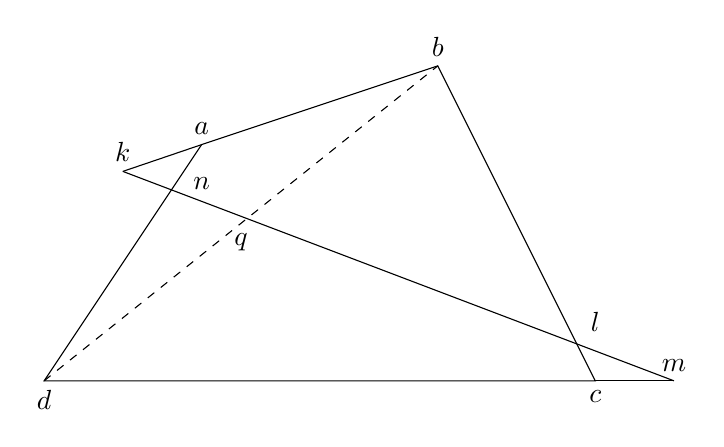
\begin{tikzpicture}[scale=1] 
    \coordinate [label=above:$a$] (a) at (2,3);
    \coordinate [label=above:$b$] (b) at (5,4);
    \coordinate [label=below:$c$] (c) at (7,0);
    \coordinate [label=below:$d$] (d) at (0,0);
    \draw (a) -- (b) -- (c) -- (d) -- cycle;
 
    \coordinate [label=above:$k$] (k) at (1,2.66);
    \coordinate [label=$n$] (n) at (2,2.3);
    \coordinate [label=below:$l$] (l) at (7,1);
    \coordinate [label=above:$m$] (m) at (8,0);
    \draw (k) -- (a);
    \draw (c) -- (m);
    \draw (k) -- (m);

    \draw [dashed] (d) -- (b);

    \coordinate [label=below:$q$] (q) at (2.5,2);
  \end{tikzpicture}    
\end{figure}

Hint: probeer hier geen analytisch bewijs te geven, er zijn teveel onbekenden.\\\\
Noem $q$ het snijpunt van $bd$ met $l$.
Beschouw nu de driehoeken $\triangle abd$ en $\triangle bcd$.
\begin{itemize}
\item Menelaos in driehoek $\triangle abd$:
  \[ (k,a,b)(q,b,d)(n,d,a) = 1 \]
\item Menelaos in driehoek $\triangle bcd$:
  \[ (l,c,m)(q,b,d)(m,d,c) = 1 \]
\end{itemize}
Merk op dat $(k,a,b)$ het omgekeerde is van $(k,b,a)$ en $(n,d,a)$ het omgekeerde van $(n,a,d)$.
\[ 1 = (l,c,m)(q,b,d)(m,d,c) = (n,a,d)(k,b,a)(l,c,d)(m,d,c) \]

\subsection*{Oefening 4}
\begin{figure}[H]
  \centering
  \begin{tikzpicture}[scale=1] 
    \coordinate [label=above:$a$] (a) at (2,3);
    \coordinate [label=above:$b$] (b) at (5,4);
    \coordinate [label=below:$c$] (c) at (7,0);
    \draw (a) -- (b) -- (c) -- cycle;

    \coordinate [label=right:$a'$] (ap) at ($ (b)!.5!(c) $);      
    \coordinate [label=below:$b'$] (bp) at ($ (c)!.5!(a) $);    
    \coordinate [label=above:$c'$] (cp) at ($ (a)!.5!(b) $);  
  
    \draw (ap) -- (a) [dashed];
    \draw (bp) -- (b) [dashed];
    \draw (cp) -- (c) [dashed];
  \end{tikzpicture}
  \caption{Voor transformatie}
\end{figure}
Er bestaat een affiene transformatie die $a$ op de oorsprong $(0,0)$ afbeeldt, $b$ op $(0,1)$ en $c$ op $(1,0)$.
Omdat de ligging van de punten $a'$, $b'$, $c'$ ten opzichte van de rechten affien invariant is, alsook de deelverhoudingen, volstaat het om de stelling te bewijzen voor de getransformeerde punten.
\begin{figure}[H]
  \centering
  \begin{tikzpicture}[scale=4] 
    \coordinate [label=below:$a$] (a) at (0,0);
    \coordinate [label=left:$b$] (b) at (1,0);
    \coordinate [label=above:$c$] (c) at (0,1);
    \draw (a) -- (b) -- (c) -- cycle;

    \coordinate [label=above:$a'$] (ap) at ($ (b)!.5!(c) $);      
    \coordinate [label=left:$b'$] (bp) at ($ (c)!.5!(a) $);    
    \coordinate [label=below:$c'$] (cp) at ($ (a)!.5!(b) $);  
  
    \draw (ap) -- (a) [dashed];
    \draw (bp) -- (b) [dashed];
    \draw (cp) -- (c) [dashed];
  \end{tikzpicture}
  \caption{Na transformatie}
\end{figure}
\begin{enumerate}
\item
  We berekenen eerst de cartesische vergelijkingen van $aa'$, $bb'$ en $cc'$:
  \[
  aa' \leftrightarrow
  \begin{pmatrix}
    x_{1} & x_{2} & 1\\
    0 & 0 & 1\\
    \nicefrac{1}{2} & \nicefrac{1}{2} & 1\\
  \end{pmatrix}
  \leftrightarrow
  x-y = 0
  \]
  \[
  bb' \leftrightarrow
  \begin{pmatrix}
    x_{1} & x_{2} & 1\\
    1 & 0 & 1\\
    0 & \nicefrac{1}{2} & 1\\
  \end{pmatrix}
  \leftrightarrow
  x+2y = 1
  \]
  \[
  cc' \leftrightarrow
  \begin{pmatrix}
    x_{1} & x_{2} & 1\\
    0 & 1 & 1\\
    \nicefrac{1}{2} &0 & 1\\
  \end{pmatrix}
  \leftrightarrow
  2x+y = 1
  \]
  Nu zijn de rechten $aa'$, $bb'$ en $cc'$ concurrent omdat de volgende determinant nul is en ze niet parallel zijn. \footnote{Zie lemma \ref{lem:rechten-concurrent-determinant}.}
  \[
  \begin{vmatrix}
    -1 & -1 & 0\\
    1 & 2 & 1\\
    2 & 1 & 1
  \end{vmatrix}
  =0
  \]
\item Bereken nu het snijpunt van $aa'$ en $cc'$: $(\nicefrac{1}{3},\nicefrac{1}{3})$, dit is het zwaartepunt.
  \[ (z,a,a') = \frac{\overrightarrow{za'}}{\overrightarrow{za}} =\frac{a'-z}{a-z} = \frac{(\nicefrac{1}{2}, \nicefrac{1}{2})-(\nicefrac{1}{3},\nicefrac{1}{3})}{(0,0)-(\nicefrac{1}{3},\nicefrac{1}{3})} = 2\]
\end{enumerate}

\subsection*{Oefening 5}
\begin{figure}[H]
  \centering
  \begin{tikzpicture}[scale=1,extended line/.style={shorten >=-#1,shorten <=-#1},extended line/.default=1cm] 
    \coordinate [label=above:$a$] (a) at (2,3);
    \coordinate [label=above:$b$] (b) at (5,4);
    \coordinate [label=below:$c$] (c) at (7,0);
    \draw (a) -- (b) -- (c) -- cycle;

    \coordinate [label=right:$a'$] (ap) at ($ (b)!.5!(c) $);      
    \coordinate [label=below:$b'$] (bp) at ($ (c)!.5!(a) $);    
    \coordinate [label=above:$c'$] (cp) at ($ (a)!.5!(b) $);  
  
    \draw (ap) -- (a) [dashed];
    \draw (bp) -- (b) [dashed];
    \draw (cp) -- (c) [dashed];

    \coordinate [label=right:$z$] (z) at ($ (a)!.6666666!(ap) $);  

    \coordinate [label=right:$p$] (p) at (7,3);
    \draw [extended line=2cm, dashed, red] (p) -- (ap);
    \draw [extended line=2cm, dashed, green] (p) -- (bp);
    \draw [extended line=2cm, dashed, blue] (p) -- (cp);
    \draw [extended line=2cm, red] (a) -- +($(p)-(ap)$) node[above,text=red] {$l_{a}$};
    \draw [extended line=2cm, green] (b) -- +($(p)-(bp)$) node[above,text=green] {$l_{b}$};
    \draw [extended line=2cm, blue] (c) -- +($(p)-(cp)$) node[above,text=blue] {$l_{c}$};
  \end{tikzpicture}
  \caption{oefening 5, een illustratie}
\end{figure}

\begin{enumerate}
\item Zij $H$ de homothetie met centrum $z$ die $a'$ afbeeldt op $a$, dan beeldt $H$ ook $b$ op $b'$ af en $c$ op $c'$.
  $H$ beeldt ook $pa'$ op $l_{a}$ af, $pb'$ op $l_{b}$ en $pc'$ op $l_{c}$.
\clarify{waarom?}
  $l_{a}$,$l_{b}$ en $l_{c}$ zijn dus concurrent.
\clarify{waarom?}
\item Omdat de afbeelding van $p$ onder $H$ $q$ is, zijn $p$, $q$ en $z$ colineair.
\item Er geldt bovendien $(z,p,q)=-2$. Zie oefening 4.
\clarify{waarom precies?}
\end{enumerate}

\extra{Oefening 6}

\subsection*{Oefening 7}
\begin{figure}[H]
  \centering
  \begin{tikzpicture}[scale=2,extended line/.style={shorten >=-#1,shorten <=-#1},extended line/.default=1cm] 
    \coordinate [label=above:$a$] (a) at (2,3);
    \coordinate [label=above:$b$] (b) at (5,4);
    \coordinate [label=below:$c$] (c) at (7,0);
    \draw (a) -- (b) -- (c) -- cycle;

    \coordinate [label=above:$p_{0}$] (p0) at ($ (a)!.7!(b) $);  
    \coordinate [label=above:$p_{1}$] (p1) at ($ (b)!.3!(c) $);  
    \coordinate [label=above:$p_{2}$] (p2) at ($ (a)!.3!(c) $);  
    \coordinate [label=above:$p_{3}$] (p3) at ($ (a)!.3!(b) $);   
    \coordinate [label=above:$p_{4}$] (p4) at ($ (b)!.7!(c) $); 
    \coordinate [label=above:$p_{5}$] (p5) at ($ (a)!.7!(c) $); 
    \coordinate [label=left:$p_{6}$] (p6) at ($ (a)!.7!(b) $);      
    \draw [extended line=1cm,dashed] (p0) -- (p1);
    \draw [extended line=1cm,dashed] (p1) -- (p2);
    \draw [extended line=1cm,dashed] (p2) -- (p3);
    \draw [extended line=1cm,dashed] (p3) -- (p4);
    \draw [extended line=1cm,dashed] (p4) -- (p5);
    \draw [extended line=1cm,dashed] (p5) -- (p6);
  \end{tikzpicture}
  \caption{oefening 7, een illustratie}
\end{figure}
Hint: probeer hier geen analytisch bewijs te geven, er zijn teveel onbekenden.\\\\

Merk de volgende zaken op:
\clarify{waarom?}
\[
\begin{array}{cc}
  (b,a,p_{0}) = (b,c,p_{1})\\
  (c,b,p_{1}) = (c,a,p_{2})\\
  \vdots\\
  (c,b,p_{4}) = (c,a,p_{5})\\
  (a,c,p_{5}) = (a,b,p_{6})\\
\end{array}
\]
Bovendien geldt het volgende:
\[ \forall p,q,r;\ (p,q,r) + (q,p,r) = 1\]
\clarify{waarom?}
Er geldt dus het volgende:
\[ (b,a,p_{0}) = (b,a,p_{6}) \Rightarrow p_{0} = p_{6} \]

\extra{Oefening 8}

\end{document}








